\chapter{系统需求分析}

\section{ 管理端功能性需求分析}

\subsection{所有功能}

管理端面对两种用户, 分别为幼儿园管理者和教师, 他们分别有不同的需求。 下面首先分析 幼儿园管理者角色所要求的功能:

\begin{itemize}

\item 注册/登录

\item 将自己的幼儿园录入系统

\begin{itemize}
	\item 幼儿园创建
	\item 删除
	\item 编辑相关信息
\end{itemize}


\item 幼儿园有自己的
\begin{itemize}
	\item 相册
	\begin{itemize}
		\item 上传
		\item 修改图片名和介绍
	\end{itemize}
	\item 云文件
	\begin{itemize}
		\item 上传
		\item 修改名字和介绍
	 	\item 创建文件夹
		\item 移动文件
	\end{itemize}
\end{itemize}


\item 发布校园通知

\item 在幼儿园录入系统后,在每个隶属于自己的幼儿园名下录入班级
\begin{itemize}
	\item 创建班级
	\item 删除
	\item 编辑相关信息
\end{itemize}

\item 每个班级都有自己的
\begin{itemize}
	\item 相册
	\item 云文件
\end{itemize}


\item 发布班级通知

\item 班级内部的人员管理

\begin{itemize}
	\item 邀请教师/学生
	\item 删除教师
	\item 教师转班
	\item 申请删除学生
	\item 申请学生转班
\end{itemize}


\item 对学生写评语

\item 如果班级和学生数量比较大, 则少数的管理者不可能承担这么多的工作, 而且管理者本身不愿意也不应当干学生数据修改等底层操作

\begin{itemize}
	\item 委派帮手
	\item 以给予手下教师不同权限的形式
	\item 比如有的教师可以做班级内的人员管理, 有的教师允许发布校园通知	
\end{itemize}
	
\end{itemize}

以上是管理者所拥有的功能, 事实上也是该系统PC管理端要提供的全部功能, 因为管理者权限最高, 应当能够使用到全部的功能。



对于教师, 分为基本功能和权限下功能。 基本功能所有教师都有, 权限下每个功能只有管理者分配了权限, 才可以拥有。

\subsection{教师基本功能}

\begin{itemize}
	\item 管理自己所在班级的
	\begin{itemize}
		\item 相册
		\item 班级文件
	\end{itemize}
	\item 发布自己所在班级通知
	\item 对自己班级内的学生写评语
\end{itemize}



\subsection{教师权限控制功能}

\begin{itemize}
	\item 校园层级上的功能
	\begin{itemize}
		\item 发布幼儿园通知
		\item 修改幼儿园基本信息 
	\end{itemize}
	   
	
	\item 班级层级上的功能
	
	\begin{itemize}
		\item 	创建班级
		\item  删除班级
		\item  编辑相关信息
	\end{itemize}
\end{itemize}



\section{社交端功能性需求分析}


社交端功能体现在手机App上, 没有用户的权限之说。 下面对社交端所需的功能做一个列表。


\begin{itemize}
	\item 不提供好友功能
	
	\item 用户自动被分入相应班级的聊天群
	
	\item 班级/学校有时间轴, 由其中父母和教师发布的状态组成
	
	\item 发布状态,可以是文字,图片或者是视频
	
	\item 看到同班 (可选为同校) 的其他父母发的状态,并且评论或者点赞
	
	\item 每个用户发布的状态会同步到该用户所在的班级和学校
	
	\item 查看
	\begin{itemize}
		\item 学校通知
		\item 班级通知
		\item 教师评语
	\end{itemize}
	
	
	\item 浏览自己孩子所在班级和学校的
	
	\begin{itemize}
		\item 相册
		\item 文件
	\end{itemize}
		
	\item 私信聊天功能
\end{itemize}


\section{业务流程需求分析}
业务流由下面的业务流图说明:

\newpage
l \newline
\begin{figure}[H]
	\centering
	\hspace*{-7cm}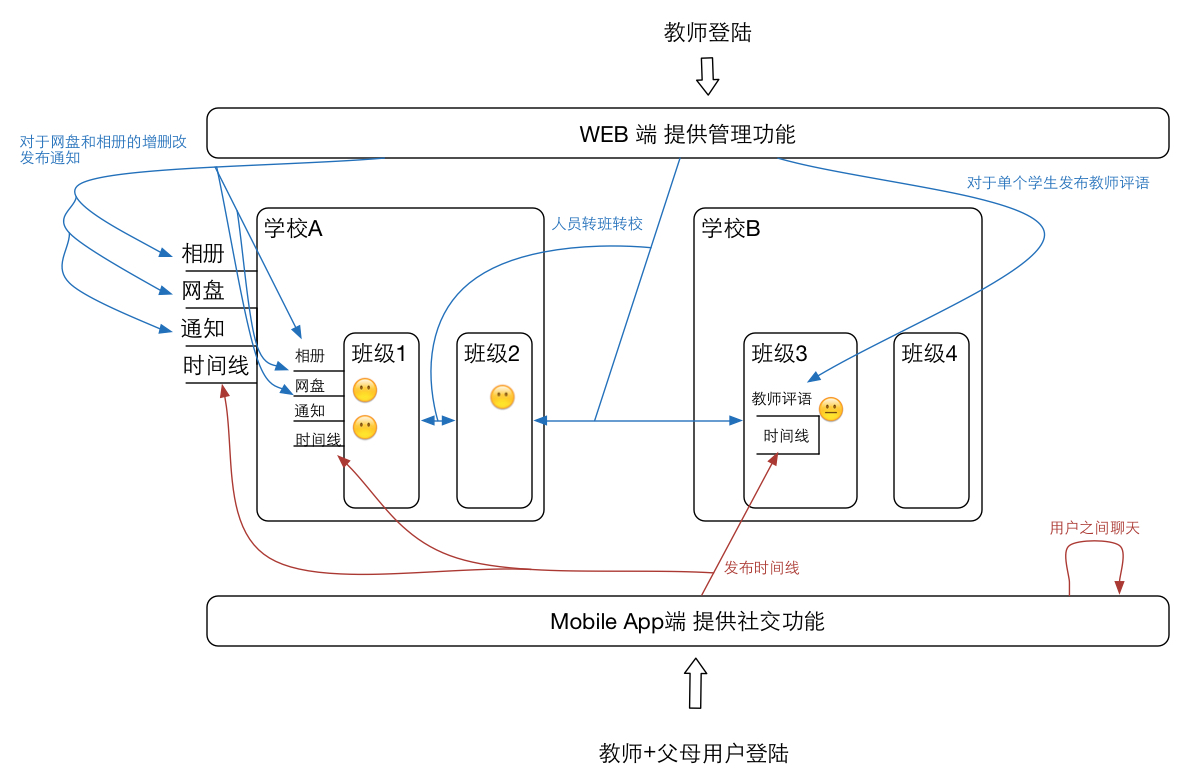
\includegraphics[width=\textwidth]{need-find.jpg}
	\figcaption{业务流图}
	\label{fig:need-find}
\end{figure}


业务流程为, 教师通过Web端登陆进行

\begin{itemize}
	\item 对于幼儿园数据的管理
	\item 发布通知
	\item 给父母发送教师评语
\end{itemize}

 父母和教师用户都可以从Mobile App端登陆
\begin{itemize}
	\item 以班级为单位的群聊
	\item 私信
	\item 发布时间线
	\item 用户的时间线可以同步在其所在的学校, 班级
\end{itemize}

\section{ 非功能性需求分析}

用户有一些非功能性的需求,下面列出来

\begin{itemize}
	

\item 保护学生用户(也就是父母)的权利

\begin{itemize}
	\item 转班,入学,从班级中删除等操作必须要通过父母的短信验证
	\item 如果是父母自行从班级中撤出, 不需要验证
\end{itemize}



\item 管理者账号有权加入任何班级群


\item 对于教师账号, 为了方便管理端的操作

\begin{itemize}
	\item 教师加入某个班级需要教师短信验证
	\item 而对于教师转班,从班级中撤出操作, 可以管理者直接操作, 不需要验证
\end{itemize}

\end{itemize}